\documentclass[12pt]{report}

\usepackage{longtable} % table
\usepackage{graphicx} % billed/image
\usepackage{hyperref} % hyperlinks
\usepackage[utf8]{inputenc} %hyperlinks
\usepackage{xcolor}
\hypersetup{
	pdfborderstyle={/S/U/W 1},
    linkbordercolor=cyan, 
    colorlinks=true,
    citebordercolor=green,     % color of links to bibliography
    filebordercolor=magenta,   % color of file links
    urlbordercolor=cyan,       % color of external links
    linkcolor=pink,
    filecolor=magenta,      
    urlcolor=cyan,
}

\begin{document}
%link start
\href{https://tex.stackexchange.com/questions/47713/underlined-links-with-hyperref-possible/220836}{Find en side hvor der kan komme streg under for den her virker ikke!!!}
%link slut
%For at lave tabler brug følgende
\begin{center}
\begin{longtable}{|c|c|c|c|}
\caption{A simple longtable example}\footnote{footnotes working fine}\\
\hline
\textbf{First entry} & \textbf{Second entry} & \textbf{Third entry} & \textbf{Fourth entry} \\
\hline
\endfirsthead
\multicolumn{4}{c}%
{\tablename\ \thetable\ -- \textit{Continued from previous page}} \\
\hline
\textbf{First entry} & \textbf{Second entry} & \textbf{Third entry} & \textbf{Fourth entry} \\
\hline
\endhead
\hline \multicolumn{4}{r}{\textit{Continued on next page}} \\
\endfoot
\hline
\endlastfoot
\multicolumn{4}{|c|}{one}\\ \hline

1 & 2 & 3 & 4 \\ 1 & 2 & 3 & 4 \\ 1 & 2 & 3 & 4 \\ 1 & 2 & 3 & 4 \\
1 & 2 & 3 & 4 \\ 1 & 2 & 3 & 4 \\ 1 & 2 & 3 & 4 \\ 1 & 2 & 3 & 4 \\
1 & 2 & 3 & 4 \\ 1 & 2 & 3 & 4 \\ 1 & 2 & 3 & 4 \\ 1 & 2 & 3 & 4 \\
1 & 2 & 3 & 4 \\ 1 & 2 & 3 & 4 \\ 1 & 2 & 3 & 4 \\ 1 & 2 & 3 & 4 \\
1 & 2 & 3 & 4 \\ 1 & 2 & 3 & 4 \\ 1 & 2 & 3 & 4 \\ 1 & 2 & 3 & 4 \\
1 & 2 & 3 & 4 \\ 1 & 2 & 3 & 4 \\ 1 & 2 & 3 & 4 \\ 1 & 2 & 3 & 4 \\
1 & 2 & 3 & 4 \\ 1 & 2 & 3 & 4 \\ 1 & 2 & 3 & 4 \\ 1 & 2 & 3 & 4 \\
1 & 2 & 3 & 4 \\ 1 & 2 & 3 & 4 \\ 1 & 2 & 3 & 4 \\ 1 & 2 & 3 & 4 \\
1 & 2 & 3 & 4 \\ 1 & 2 & 3 & 4 \\ 1 & 2 & 3 & 4 \\ 1 & 2 & 3 & 4 \\
1 & 2 & 3 & 4 \\ 1 & 2 & 3 & 4 \\ 1 & 2 & 3 & 4 \\ 1 & 2 & 3 & 4 \\
1 & 2 & 3 & 4 \\ 1 & 2 & 3 & 4 \\ 1 & 2 & 3 & 4 \\ 1 & 2 & 3 & 4 \\
1 & 2 & 3 & 4 \\ 1 & 2 & 3 & 4 \\ 1 & 2 & 3 & 4 \\ 1 & 2 & 3 & 4 \\
\end{longtable}
\end{center} 
%tabel slut
\newpage
%husk at det er det rigtige navn og lig filen i mappen eller lav en ny mappe med filen og skriv den før fil navnet. sæt billedet ind og skriv en note hvis der skal gøres noget ved det senere. 
%billed start
\begin{figure}
  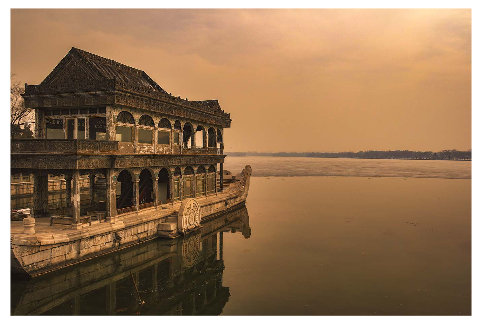
\includegraphics[width=\linewidth]{boat.png} 
  \caption{A boat.}
  \label{fig:boat1}
\end{figure}

Figure \ref{fig:boat1} shows a boat.
%billed slut 
\newpage
%enum start
\begin{enumerate}
\item Dette er for tal\footnote{brug \textbackslash footnotes til at lave footnotes}
\item husk der skal stå \textbackslash item først
\begin{enumerate}
\item bare skriv flere af de samme enumerate 
\item så vil det stå på denne måde 
\begin{itemize}
\item ellers kan der også bruges itemize
\end{itemize}
\end{enumerate}
\end{enumerate}
 \newpage 
 \href{https://www.overleaf.com/learn/latex/Hyperlinks} {hyperlinks} \\ \\
 \url{https://www.overleaf.com/learn/latex/Hyperlinks}
\end{document}
%enum slut